


\subsection{Design and Implementation}

\subsubsection{Class Diagrams}

As stated in section ~\ref{section:aims}, this project extends from SICSA project which uses only publications as expertise evidence.
The aim of this project is to integrate funded projects with publications to improve the performance of the retrieval.
Figure ~\ref{fig:classDiagram1} shows the relationship between Candidate, Project, Publication and University classes. Each component in the figure
shows only important attributes and methods. The Candidate class represents an expert who lectures at a university and has a set of publications and projects.
\begin{figure}
\centering
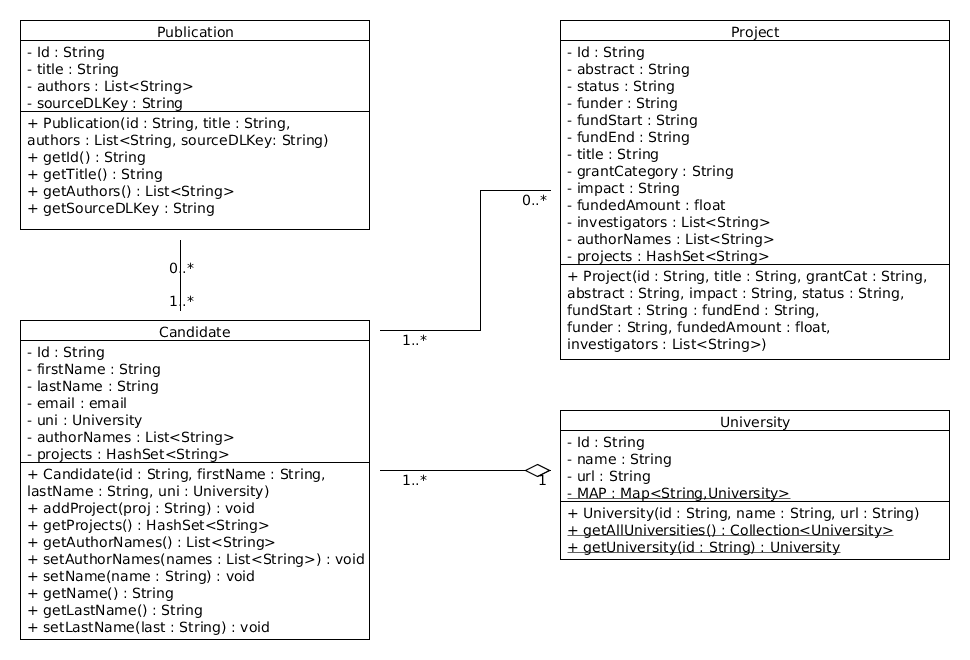
\includegraphics[scale=0.4]{./figures/classDiagram1.png}
\caption{Class Diagram} \label{fig:classDiagram1} 
\end{figure}

As stated in section ~\ref{section:goodexpert}, the features extracted from funded projects and publications of each expert will be used in Learning to Rank
to improve the retrieval performance of the system. But before we get to Learning to Rank, first of all, we need to understand
AcademTechQuerying Class and RetrievedResults Class which are components used in retrieving results with respect to a query. 
\begin{figure}
\centering
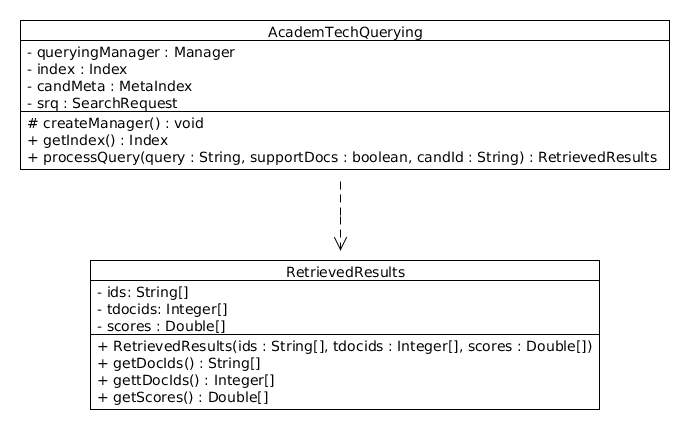
\includegraphics[scale=0.4]{./figures/AcademTechQuerying.png}
\caption{AcademTechQuerying Class and RetrievedResults Class} \label{fig:AcademTechQuerying} 
\end{figure}

Figure ~\ref{fig:AcademTechQuerying} shows class diagrams of AcademTechQuerying and RetrievedResults. As stated in section ~\ref{section:terrier},
the search engine platform used in this project is Terrier. It handles indexing and retrieval processes discussed in section ~\ref{section:IRarchitecture}.
The AcademTechQuerying Class makes use of 2 Terrier components as follows:  
\begin{itemize}
 \item queryingManager of type Manager, responsible for handling/co-ordinating the main high-level operations of a query.
 \item srq of type SearchRequest, responsible for retrieving search result from Manager.
\end{itemize}
The important method of AcademTechQuerying is processQuery(). It returns RetrievedResults. This method takes a query string, supportDocs and candId as arguments. The first argument tells
the system that a query is used to retrieve the result, the second and third arguments are used in case the system wants documents associated to a candidate 
with respect to a query.

The RetrievedResults Class has 3 attributes as follows:
\begin{itemize}
 \item ids, an array of String, which is the ids of the documents(in this case, ids of experts) retrieved by the system.
 \item tdocids, an array of Integer, which is the ids used by Terrier
 \item scores, an array of Double, which is the scores of each document retrieved by the system.
\end{itemize}

\subsubsection{Data Extraction}
\begin{figure}
\centering
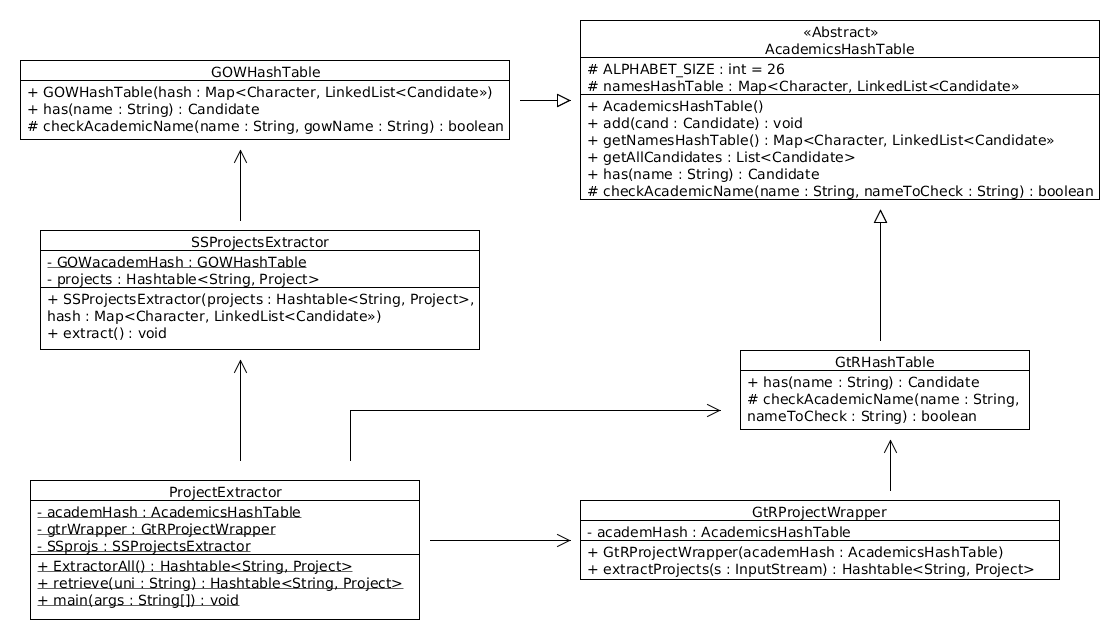
\includegraphics[scale=0.35]{./figures/projectsExtraction.png}
\caption{Projects Extraction Class Diagrams} \label{fig:projectsExtraction} 
\end{figure}
In section ~\ref{section:aims}, it was stated that funded project information are obtained from Grant on the Web~\cite{gow} and Research Councils UK~\cite{gtr}.
This section shows classes used to extract funded projects from each source and gives statistics regarding the number of total funded projects from each source.
Figure ~\ref{fig:projectsExtraction} shows class diagram related to projects extraction.
\paragraph{AcademicsHashTable} is an abstract class which makes use of HashMap data structure, Map<Character, LinkedList<Candidate>>, for efficient look up when matching candidate to our
known candidates. It is keyed by the first character of candidate's name. There are 2 abstract methods in this class: has() and checkAcademicName() methods.
Both of them are used together to check if the candidate from a source is matched to our known candidates.
\paragraph{GtRHashTable} extends from the abstract class AcademicsHashTable. The purpose of this class is the same as AcademicsHashTable Class but
implements has() and checkAcademicName() methods which are suitable for data in Research Councils UK~\cite{gtr}.
\paragraph{GOWHashTable} extends from the abstract class AcademicsHashTable. Its purpose is similar to AcademicsHashTable Class but
has different implementations of hash() and checkAcademicName() methods to GOWHashTable's which is suitable for Grant on the Web~\cite{gow} spreadsheet.
\paragraph{SSProjectsExtractor} is a class that makes use of GOWHashTable Class to extract funded projects from Grant on the Web~\cite{gow} spreadsheet.
\paragraph{GtRProjectWrapper} is a class used GOWHashTable Class to extract funded projects from Research Councils UK~\cite{gtr}.
\paragraph{ProjectExtractor} is a class that makes use of SSProjectsExtractor and GtRProjectWrapper Classes to extract funded projects from both sources.

\begin{table}
\centering
\begin{tabular}{|c|c|}
\hline \textbf{Source} & \textbf{Number of Funded Projects} \\
\hline Grant on the Web & 32 \\
\hline Research Councils UK & 337 \\
\hline   & 369 total \\ 
\hline
\end{tabular}
\caption{The number of funded projects extracted from each source} \label{table:stats}
\end{table}
Figure ~\ref{table:stats} shows the number of funded projects extracted from each source. There are 1569 known candidates in the system.

\subsubsection{Retrieving Documents (Experts) with respect to a Query} \label{section:union}

\begin{figure}
\centering
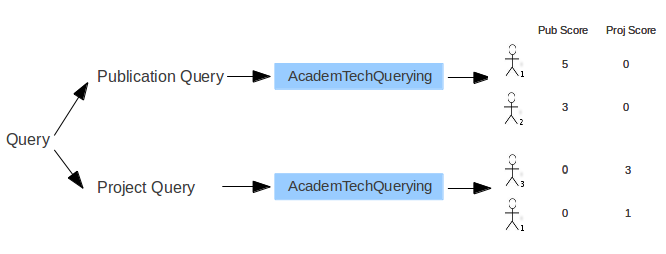
\includegraphics[scale=0.7]{./figures/querying.png}
\caption{Querying} \label{fig:quering} 
\end{figure}
\quad
\begin{figure}
\centering
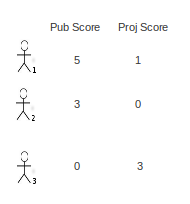
\includegraphics[scale=0.7]{./figures/union.png}
\caption{Results After Union} \label{fig:union} 
\end{figure}
Figure ~\ref{fig:quering} shows the process of obtaining documents (experts) with respect to a query. 
First of all, the user query is transformed into publication query and project
query. AcademTechQuerying Class then processes both queries to get results with respect to publication query and project query. The results of both
queries are then unioned as shown in Figure ~\ref{fig:union}.

\subsubsection{Producing a Learned Model}
Section ~\ref{section:learnedmodel} described general steps to produce a learned model. This section aims to discuss classes involved in producing a learned model.
As section ~\ref{section:learnedmodel} suggested, the first step in producing a learned model is to generate a set of training queries. 
Then all features described in Section ~\ref{section:goodexpert} for each document (expert) with respect to each training query are extracted and saved
in a file. This file in learning to rank is called LETOR file.
34 training queries~\ref{table:trainingqueries} are trained by the tool called RankLib~\ref{section:rankLib} to get a learned model. This process is done 
only one time. Once a learned model is obtained, for every query, the model is applied to generate a final ranking.
\begin{table}
\centering
\begin{tabular}{|c|l|c|l|}
\hline \textbf{\#} & \textbf{Query} & \textbf{\#} & \textbf{Query} \\
\hline 1 & language modelling & 18 & game theory\\
\hline 2 & manets & 19 & stable marriage \\
\hline 3  & match & 20 & quantum computation\\ 
\hline 4  & multimodal & 21 & constraint modelling\\ 
\hline 5  & music as navigation cues & 22 & home networks\\ 
\hline 6  & networking security & 23 & wireless sensor networks\\ 
\hline 7  & neural network & 24 & distributed systems\\ 
\hline 8  & older adults use of computers & 25 & operating system\\ 
\hline 9  & parallel logic programming & 26 & terrier\\ 
\hline 10  & query expansion & 27 & text searching\\ 
\hline 11  & road traffic accident statistics & 28 & trec collection class\\ 
\hline 12  & shoogle & 29 & usability\\ 
\hline 13  & skill-based behavior & 30 & utf support terrier\\ 
\hline 14  & sound in multimedia human-computer interfaces & 31 & visual impairment\\ 
\hline 15  & statistical inference & 32 & wafer fab cost \\ 
\hline 16  & suffix tree & 33 & database\\ 
\hline 17  & mobile hci & 34 & programming languages\\ 
\hline
\end{tabular}
\caption{Training Queries} \label{table:trainingqueries}
\end{table}

\begin{figure}
\centering
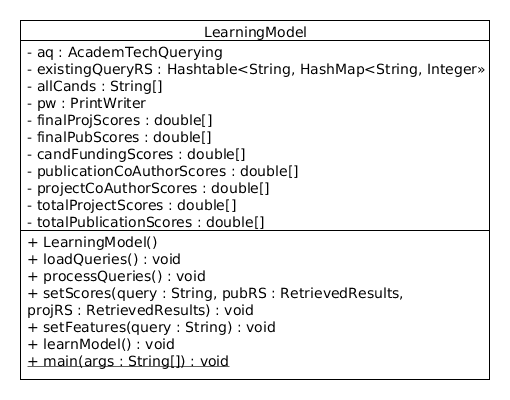
\includegraphics[scale=0.7]{./figures/learningModel.png}
\caption{Class Diagram of LearningModel} \label{fig:learningmodel} 
\end{figure}

Figure ~\ref{fig:learningmodel} shows a class diagram that is used to produce a learned model. There are 5 important methods as follows
\begin{itemize}
 \item loadQueries() is a method that loads all training queries from a file.
 \item processQuery() is a method that retrieve documents (experts) with respect to publication query and project query.
 \item setScores() is a method that performs a union between results with respect to publication query and project query as discussed in Section ~\ref{section:union}
 \item setFeatures() is a method that extracts features for each document (expert) and write into a LETOR file.
 \item learnModel() is a method that produces a learned model using RankLib~\ref{section:rankLib}.
\end{itemize}

As stated in Section ~\ref{section:rankLib}, learning to rank algorithms used in this project are AdaRank and Coordinate Ascent. The performance of each
of them will be discussed in Evaluation Section.

\subsubsection{Applying a Learned Model}
Now that a learned model has been generated, this learned model can be applied to produce optimal ranking. Basically, when 







